\scanpage{20}
\mspage{\handwritten{11}}
\[
\operatorname{card}Y_t(k')\equiv c_t+(-1)^{n-1}\operatorname{Tr}f_t\,,
\]
où \deleted{\unsure{x}}
\[
c_t=\handwritten{\sum_{0\leq i\leq n-1}(-1)^i}\operatorname{Trace}\text{ de }\operatorname{Frob}_{k'}\text{ opérant sur }H^i(X,\underline{O}_X)\,,
\]
et où $f_t$ est l'élément du groupe \inserted{\handwritten{quotient}} $G_o=\operatorname{Aut}_{\underline{F}_p}(V_o)$ de \handwritten{$\pi$}, \deleted{\unsure{qui est}} image de l'\unsure{\deleted{é}E|É|E}lément de frobenius de \handwritten{$\pi$} associé au point \deleted{fermé} $t\handwritten{\in}U(k')$. Quitte à passer à\inserted{remplacer d'abord $k$ par} une extension finie, \deleted{\unsure{de k}} de sorte que \deleted{\unsure{les valeurs}} $\operatorname{\unsure{\deleted{f}F|f}rob}_k$ opérant sur les $H^i(X,\underline{O}_X)$ soit à valeurs propres toutes égales à 0 ou 1, on peut supposer que $c_t$ est indépendant de $t$, \inserted{soit $c$.} Il résulte alors de 7.1 qu'il existe un élément $f$ de $G_o$ tel que $c+(-1)^{n-1}\operatorname{Tr}f\unsure{\equiv|=\deleted{x}}a\bmod p$, et il suffit donc de choisir un $t\handwritten{\in}U$ (considéré comme élément de $U(k(t))$ de telle façon que $f_t=f$. Mais ceci est possible en vertu du théorème de \rlap{\handwritten{\v{\phantom{C}}}}Cebotâref.

\margin{\figure{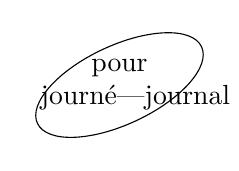
\begin{tikzpicture}\draw[rotate=25] (0,0) ellipse (1.15cm and 0.5cm);\node[text width=2cm,align=center] at (0,0) {\handwritten{pour \unsure{journé|journal}}};\end{tikzpicture}}}
\uline{Corollaire} 7.3. \inserted{(Si $n$ pair\inserted{\handwritten{$\geq4$}}, $X$ lisse).} On peut trouver un ouvert $U'$ \inserted{\handwritten{(\unsure{variété|ouvert} de la grassmannienne des droites)\deleted{de}}} de $S_d$, tel que pour toute droite \inserted{\handwritten{$D\in U'(k')$}} de $\handwritten{(}S_d\handwritten{)_{k'}}$ \deleted{qui rencontre \unsure{un|U}\handwritten{\unsure{\varnothing|k}} et qui définit}\inserted{\handwritten{$D$ est}} un pinceau de Lefschetz sur $X_{\handwritten{k'}}$, si $t$ désigne le point générique de cette droite, le motif $E(Y_t)$ des \deleted{\unsure{s}}cycles évanescents sur $Y_t$ \deleted{\unsure{soit de}} ne soit pas de niveau 1 (donc ne contienne pas de sous-motif $\handwritten{\ne}0$ de niveau 1, pas même sur une extension de $k(t)$, d'après le résultat de simplicité rappelé au n°6).
\margin{\handwritten{($k'$ une ext. qqle. de $k$)}}

On prend $U$ comme dans la démonstration de 7.2, \inserted{\handwritten{et tel que les $Y_s$ $(s\in U)$ soient lisses.}} On peut (grâce au fait qu'un motif de niveau $\handwritten{\leq}\deleted{\unsure{\leq}}1$ se spécialise en un motif de niveau $\handwritten{\leq}1$, comme on a signalé au n°6 comme conséquence du critère de Ogg-Néron-Chafarévitch) supposer que $k$ est fini, et \unsure{il|on} \deleted{\unsure{est ramené à prouver que}} suffit de prouver que l'on peut trouver un point fermé $s$ de $D\handwritten{\cap U}$ tel que les valeurs propres de Frobenius opérant sur $E^{n-1}(Y_s,\underline{Q}_{\handwritten{\unsure{\ell|l}}})$ ($\handwritten{\ell}$ un nombre premier fixé $\handwritten{\ne\ell}$) ne soient pas toutes divisibles par $p$. Or le nombre de points de $Y_t$ est égal à la somme alternée des traces de frobenius opérant sur les \deleted{\handwritten{\unsure{$H$}}}
\margin{\figure{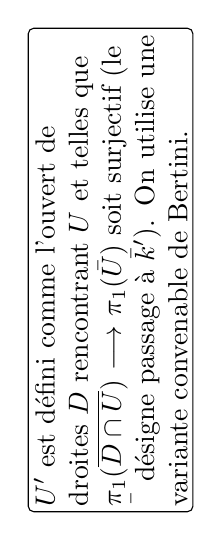
\begin{tikzpicture}\node[draw,rounded corners=2pt,rotate=90,text width=6cm,align=left,inner sep=2pt] {\handwritten{$U'$ est défini comme \unsure{l'ouvert} de droites \inserted{$D$} rencontrant $U$ et telles que $\pi_1(\overline{D\cap U})\longrightarrow\pi_1(\bar U)$ soit surjectif (le $\bar{\phantom{k}}$ désigne passage à $\bar{k}'$). On utilise une \uline{variante} \unsure{convenable} de Bertini.}};\end{tikzpicture}}}
% archive sheet number: 19
